\documentclass[a4paper,14pt]{extarticle}

% Путь до папки с общими шаблонами
\newcommand{\pathToCommonFolder}{/home/denilai/Documents/repos/latex/Common}
% Название работы в титуле
\newcommand{\workname}{Отчет по практической работе №4}
% Название дисциплины в титуле
\newcommand{\discipline}{Архитектура процессоров и микропроцессоров}
% Название кафедры в титуле
\newcommand{\kafedra}{Кафедра вычислительной техники}
% Тема работы в титуле
\newcommand{\theme}{Стадии выполнения команд процессором КР580ВМ80}
% Должность преподавателя в титуле
\newcommand{\rang}{cтарший преподаватель кафедры ВТ}
% ФИО преподавателя в титуле
\newcommand{\teacherfio}{Ю.~М.Скрябин}
\newcommand{\studentfio}{К.~Ю.~Денисов}
\newcommand{\signature}{\pathToCommonFolder/denisov-signature}

\newcommand{\pt}{PacketTracer\copyright}

\usepackage{tabularx}

\newcommand{\router}{R1\_DENISOV~}
\newcommand{\switch}{S1~}



\usepackage{booktabs}
\newcolumntype{b}{X}
\newcolumntype{s}{>{\hsize=.5\hsize}X}
\newcommand{\heading}[1]{\multicolumn{1}{|c|}{#1}}

% установка размера шрифта для всего документа
%\fontsize{20pt}{18pt}\selectfont
\usepackage{extsizes} % Возможность сделать 14-й шрифт

% Вставка заготовки преамбулы
% Этот шаблон документа разработан в 2014 году
% Данилом Фёдоровых (danil@fedorovykh.ru) 
% для использования в курсе 
% <<Документы и презентации в \LaTeX>>, записанном НИУ ВШЭ
% для Coursera.org: http://coursera.org/course/latex .
% Исходная версия шаблона --- 
% https://www.writelatex.com/coursera/latex/5.3

% В этом документе преамбула

% Для корректного использования русских символов в формулах
% пакеты hyperref и настройки, связанные с ним, стоит загуржать
% перед загрузкой пакета mathtext



% поддержка русских букв
% кодировка шрифта
%\usepackage[T2A]{fontenc} 
\usepackage{pscyr}

% использование ненумеровонного абзаца с добавлением его в содержаниеl

\newcommand{\anonsection}[1]{\section*{#1}\addcontentsline{toc}{section}{#1}}
\newcommand{\sectionunderl}[1]{\section*{\underline{#1}}}


% настройка окружения enumerate
\usepackage{enumitem}
\setlist{noitemsep}
\setlist[enumerate]{labelsep=*, leftmargin=1.5pc}

\usepackage{hyperref}

% сначала ставить \usepackage{extsizes} % Возможность сделать 14-й шрифт
% для корректной установки полей вставлять преамбулу следует в последнюю очередь (но перед дерективой замены \rmdefault)
\usepackage[top=20mm,bottom=25mm,left=35mm,right=20mm]{geometry} % Простой способ задавать поля

\hypersetup{				% Гиперссылки
	unicode=true,           % русские буквы в раздела PDF
	pdftitle={Заголовок},   % Заголовок
	pdfauthor={Автор},      % Автор
	pdfsubject={Тема},      % Тема
	pdfcreator={Создатель}, % Создатель
	pdfproducer={Производитель}, % Производитель
	pdfkeywords={keyword1} {key2} {key3}, % Ключевые слова
	colorlinks=true,       	% false: ссылки в рамках; true: цветные ссылки
	linkcolor=red,          % внутренние ссылки
	citecolor=black,        % на библиографию
	filecolor=magenta,      % на файлы
	urlcolor=blue           % на URL
}

%%% Работа с русским языком
\usepackage{cmap}					% поиск в PDF
\usepackage{mathtext} 				% русские буквы в формулах
\usepackage[T2A]{fontenc}			% кодировка
\usepackage[utf8]{inputenc}			% кодировка исходного текста
\usepackage[english,russian]{babel}	% локализация и переносы
\usepackage{indentfirst}
\frenchspacing

%для изменения названия списка иллюстраций
\usepackage{tocloft}


\renewcommand{\epsilon}{\ensuremath{\varepsilon}}
\renewcommand{\phi}{\ensuremath{\varphi}}
\renewcommand{\kappa}{\ensuremath{\varkappa}}
\renewcommand{\le}{\ensuremath{\leqslant}}
\renewcommand{\leq}{\ensuremath{\leqslant}}
\renewcommand{\ge}{\ensuremath{\geqslant}}
\renewcommand{\geq}{\ensuremath{\geqslant}}
\renewcommand{\emptyset}{\varnothing}

% Изменения параметров списка иллюстраций
\renewcommand{\cftfigfont}{Рисунок } % добавляем везде "Рисунок" перед номером
\addto\captionsrussian{\renewcommand\listfigurename{Список иллюстративного материала}}

\newcommand{\tm}{\texttrademark\ }
\newcommand{\reg}{\textregistered\ }


%%% Дополнительная работа с математикой
\usepackage{amsmath,amsfonts,amssymb,amsthm,mathtools} % AMS
\usepackage{icomma} % "Умная" запятая: $0,2$ --- число, $0, 2$ --- перечисление

%% Номера формул
%\mathtoolsset{showonlyrefs=true} % Показывать номера только у тех формул, на которые есть \eqref{} в тексте.
%\usepackage{leqno} % Нумереация формул слева

%% Свои команды
\DeclareMathOperator{\sgn}{\mathop{sgn}}

%% Перенос знаков в формулах (по Львовскому)
\newcommand*{\hm}[1]{#1\nobreak\discretionary{}
{\hbox{$\mathsurround=0pt #1$}}{}}


% отступ для первого абзаца главы или параграфа
%\usepackage{indentfirst}

%%% Работа с картинками
\usepackage{graphicx}  % Для вставки рисунков
\graphicspath{{images/}{screnshots/}}  % папки с картинками
\DeclareGraphicsExtensions{.pdf,.png,.jpg}
\setlength\fboxsep{3pt} % Отступ рамки \fbox{} от рисунка
\setlength\fboxrule{1pt} % Толщина линий рамки \fbox{}
\usepackage{wrapfig} % Обтекание рисунков текстом

%%% Работа с таблицами
\usepackage{array,tabularx,tabulary,booktabs} % Дополнительная работа с таблицами
\usepackage{longtable}  % Длинные таблицы
\usepackage{multirow} % Слияние строк в таблице

%%% Теоремы
\theoremstyle{plain} % Это стиль по умолчанию, его можно не переопределять.
\newtheorem{theorem}{Теорема}[section]
\newtheorem{proposition}[theorem]{Утверждение}

\theoremstyle{plain} % Это стиль по умолчанию, его можно не переопределять.
\newtheorem{work}{Практическая работа}[part]


 
 
\theoremstyle{definition} % "Определение"
\newtheorem{corollary}{Следствие}[theorem]
\newtheorem{problem}{Задача}[section]
 
\theoremstyle{remark} % "Примечание"
\newtheorem*{nonum}{Решение}



%%% Программирование
\usepackage{etoolbox} % логические операторы

%%% Страница

%	\usepackage{fancyhdr} % Колонтитулы
% 	\pagestyle{fancy}
%   \renewcommand{\headrulewidth}{0pt}  % Толщина линейки, отчеркивающей верхний колонтитул
% 	\lfoot{Нижний левый}
% 	\rfoot{Нижний правый}
% 	\rhead{Верхний правый}
% 	\chead{Верхний в центре}
% 	\lhead{Верхний левый}
%	\cfoot{Нижний в центре} % По умолчанию здесь номер страницы

\usepackage{setspace} % Интерлиньяж
\onehalfspacing % Интерлиньяж 1.5
%\doublespacing % Интерлиньяж 2
%\singlespacing % Интерлиньяж 1

\usepackage{lastpage} % Узнать, сколько всего страниц в документе.

\usepackage{soul} % Модификаторы начертания


\usepackage[usenames,dvipsnames,svgnames,table,rgb]{xcolor}


\usepackage{csquotes} % Еще инструменты для ссылок

%\usepackage[style=authoryear,maxcitenames=2,backend=biber,sorting=nty]{biblatex}

\usepackage{multicol} % Несколько колонок

\usepackage{tikz} % Работа с графикой
\usepackage{pgfplots}
\usepackage{pgfplotstable}

% модуль для вставки рыбы
\usepackage{blindtext}

\usepackage{listings}
\usepackage{color}


% для поворота отдельной страницы. Использовать окружение \landscape
\usepackage{pdflscape} 
\usepackage{rotating} 


\definecolor{mygreen}{rgb}{0,0.6,0}
\definecolor{mygray}{rgb}{0.5,0.5,0.5}
\definecolor{mymauve}{rgb}{0.58,0,0.82}


% пример импорта файла
%\lstinputlisting{/home/denilai/repomy/conf/distributions}

\lstset{
	language=Python,
	basicstyle=\footnotesize,        % the size of the fonts that are used for the code
	numbers=left,                    % where to put the line-numbers; possible values are (none, left, right)
	numbersep=5pt,                   % how far the line-numbers are from the code
	numberstyle=\tiny\color{mygray}, % the style that is used for the line-numbers
	stepnumber=2,                    % the step between two line-numbers. If it's 1, each line will be numbered
	% Tab - 2 пробела
	tabsize=2,    
	% Автоматический перенос строк
	breaklines=true,
	frame=single,
	breakatwhitespace=true,
	title=\lstname 
}



\author{Кирилл Денисов ИВБО-02-19}
\title{Практическая работа №8\\Вариант 6}
\date{\today}

\renewcommand{\withouttheme}{1}

% установка полуторного интервала
% \usepackage{setspace}  
% \onehalfspacing

% использовать Times New Roman
\renewcommand{\rmdefault}{ftm}


\begin{document}
	%\thispagestyle{empty}
	% Вставка первого титульного листа
	%%\newcommand{\withouttheme}{} добавить эту переменную для определения, нужна ли тема
%     {} - нужна
%    {1} - не нужна

%\newcommand{\withoutsubmissiondate}{} добавить эту переменную для определения, нужен ли срок предоставления отчета
%     {} - нужен
%    {1} - не нужен
\begin{center}
	\begin{figure}[h!]
		\begin{center}
		
\includegraphics[width=0.17\linewidth]{\pathToCommonFolder/gerb}
		%\caption{}\label{pic:first}
		%	\vspace{5ex}
		\end{center}	
	\end{figure}
 	\small	МИНОБРНАУКИ РОССИИ \\
	Федеральное государственное бюджетное образовательное учреждение\\
						высшего профессионального образования\\
\normalsize					
\textbf{«МИРЭА – Российский технологический университет»\\
						РТУ МИРЭА}\\
						\noindent\rule{1\linewidth}{1pt}\\
       Институт информационных технологий\\ %\vspace{2ex}
					\kafedra\\
		\vspace{3ex}
			\large \textbf{\workname}  \\
		%\vspace{1ex}
						по дисциплине\\ «\discipline» \\
		\vspace{3ex}
		\if \withouttheme
			\textbf{Тема работы:}\\ <<\theme>>
		\fi
\vspace{3ex}
\small
\begin{table}[h!]
\begin{tabular}{p{0.14\linewidth}p{0.38\linewidth}p{0.25\linewidth}p{0.2\linewidth}}
	\textbf{Выполнил:} & студент группы ИВБО-02-19 & \studentfio &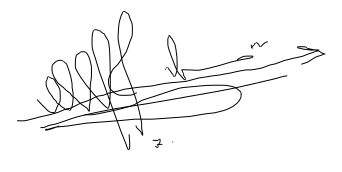
\includegraphics[width=0.8\linewidth]{\signature}\\ \\
	\textbf{Принял:} & \rang & \teacherfio 
\end{tabular}
\end{table}
\end{center}

\begin{flushleft}
	\begin{tabular}{p{0.25\linewidth}l}

		Работа выполена & <<\noindent\rule{2em}{1pt}>>
		                    \noindent\rule{5em}{1pt} 202\noindent\rule{1em}{1pt} \\

		<<Зачтено>> & <<\noindent\rule{2em}{1pt}>>
		\noindent\rule{5em}{1pt} 202\noindent\rule{1em}{1pt} \\

	\end{tabular}
\end{flushleft}

\normalsize
\begin{center}	
\vfill 
Москва 2021
\end{center}

	\newpage
	%\tableofcontents
	\newpage
	%\listoftables
\maketitle


\begin{table}[htbp]
	\begin{center}
		\caption{Таблица адресации}
		\begin{tabular}{|l|l|l|l|m{0.17\linewidth}|}
			\hline\
			\textbf{Устройство}  & \textbf{Интерфейс} & \textbf{IP-адрес} & \textbf{Маска подсети} & \textbf{Шлюз по умолчанию} \\ \hline
			\router & G0/1   & 192.168.1.6  & 255.255.255.0  &  —          \\\hline
			\switch & VLAN 1 & 192.168.1.16 & 255.255.255.0  & 192.168.1.6 \\\hline
			PC-A    & NIC    & 192.168.1.26  & 255.255.255.0 & 192.168.1.6\\\hline
		\end{tabular}
		\label{tab:adress}
	\end{center}
\end{table}

\begin{mypart}{Настройка основных параметров устройств}
	
	\begin{step}{Создание сети согласно топологии}
		
		Создадим сеть для выполнения данного практического задания согласно топологии. (см. рисунок \ref{fig:pr8-topology}).
		% TODO: \usepackage{graphicx} required
		\begin{figure}[h!]
			\centering
			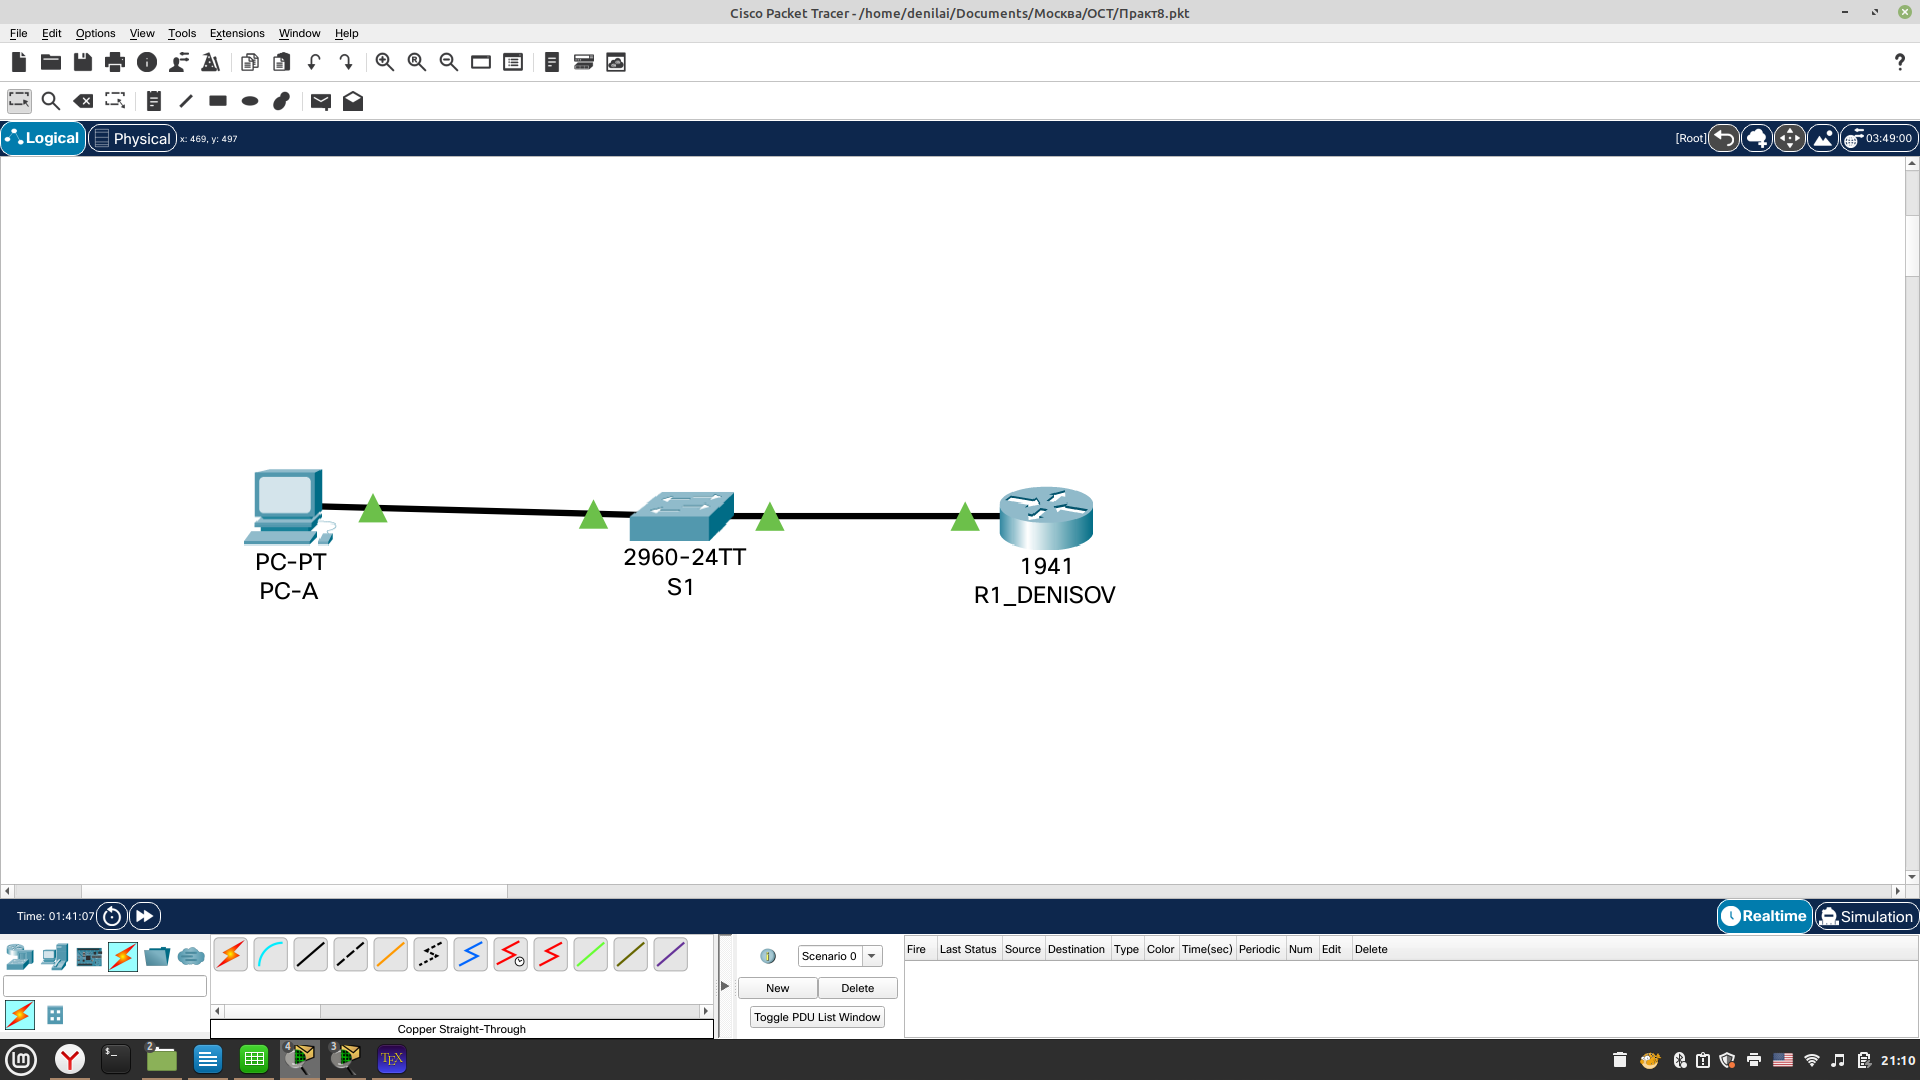
\includegraphics[width=1\linewidth]{images/pr8-topology}
			\caption{Топология сети}
			\label{fig:pr8-topology}
		\end{figure}
		
	\end{step}

\begin{step}{Выполнение инициализации и перезагрузки маршрутизатора и коммутатора}
	
	Дождемся инициализации маршрутизатора  и коммутатора S1 и выполним их перезагрузку.
	
\end{step}

\begin{step}{Настройка маршрутизатора}
	
	Подключимся к маршрутизатору \router и произведем его настройку в соответствии с заданием. Приведем текущую конфигурацию маршрутизатора. 
	\begin{lstlisting}
		R1_DENISOV#show running-config 
		Building configuration...
		
		Current configuration : 1211 bytes
		!
		version 15.1
		no service timestamps log datetime msec
		no service timestamps debug datetime msec
		service password-encryption
		security passwords min-length 10
		!
		hostname R1_DENISOV
		!
		login block-for 30 attempts 2 within 120
		!
		enable secret 5 $1$mERr$5wXi8fVAu3dNc0gNCjvIQ1
		!
		ip cef
		no ipv6 cef
		!
		username SSHadmin privilege 15 secret 5 $1$mERr$uMzC7If3IbCZVifeGQ3rg/
		!
		license udi pid CISCO1941/K9 sn FTX15244MJ5-
		!
		ip domain-name cisco-lab.ru
		!
		spanning-tree mode pvst
		!
		interface GigabitEthernet0/0
		no ip address
		duplex auto
		speed auto
		shutdown
		!
		interface GigabitEthernet0/1
		ip address 192.168.1.6 255.255.255.0
		duplex auto
		speed auto
		!
		interface Vlan1
		no ip address
		shutdown
		!
		ip classless
		!
		ip flow-export version 9
		!
		ip access-list extended sl_def_acl
		deny tcp any any eq telnet
		deny tcp any any eq www
		deny tcp any any eq 22
		permit tcp any any eq 22
		!
		banner motd ^CAuthorized users only!^C
		!
		line con 0
		exec-timeout 5 0
		password 7 0822455D0A16
		login
		!
		line aux 0
		!
		line vty 0 4
		exec-timeout 5 0
		password 7 0822455D0A16
		login local
		transport input ssh
	    !
		end
	\end{lstlisting}
	
	После проведения настройки сохраним текущую конфигурацию в файл загрузочной конфигурации с помощью команды \texttt{copy running-config startup-config}.
\end{step}

\begin{step}{Установка более надежных паролей}
	
	Согласно данным рекомендациям по лучшим практическим методикам надежные
	пароли, примеры которых приведены в этой лабораторной работе, необходимо всегда использовать в
	реальной работе. Однако для упрощения выполнения работы в остальных лабораторных работах
	данного курса используются пароли cisco и class.
	
	Измените зашифрованный пароль привилегированного режима EXEC в соответствии с
	рекомендациями. Установите следующий пароль: \textbf{Enablep@55} с помощью команды \texttt{enable secret Enablep@55}.
	
	Установим минимальную длину 10 символов для всех паролей с помощью команды \texttt{ security passwords min-length 10}.
\end{step}

\begin{step}{Настройка компьютер PC-A}
	Настроим для PC-A IP-адрес и маску подсети и шлюз по умолчанию в соответствии с заданием, приведенным в  таблице \ref*{tab:adress} (см. рисунок \ref{fig:pr8-pc-a}).
	
	% TODO: \usepackage{graphicx} required
	\begin{figure}[h!]
		\centering
		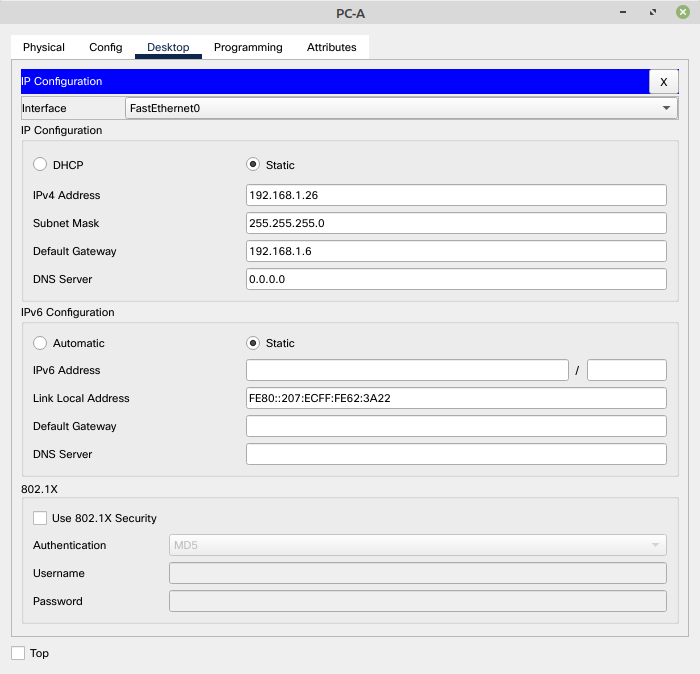
\includegraphics[width=0.6\linewidth]{images/pr8-pc-a}
		\caption{}
		\label{fig:pr8-pc-a}
	\end{figure}
	
\end{step}

\begin{step}{Проверка подключения к сети}
	
	Пошлем с PC-A эхо-запрос на маршрутизатор \router. Убедимся, что эхо-запрос выполнен
	успешно (см. рисунок \ref{fig:pr8-ping-router}).
	
	
	% TODO: \usepackage{graphicx} required
	\begin{figure}[h!]
		\centering
		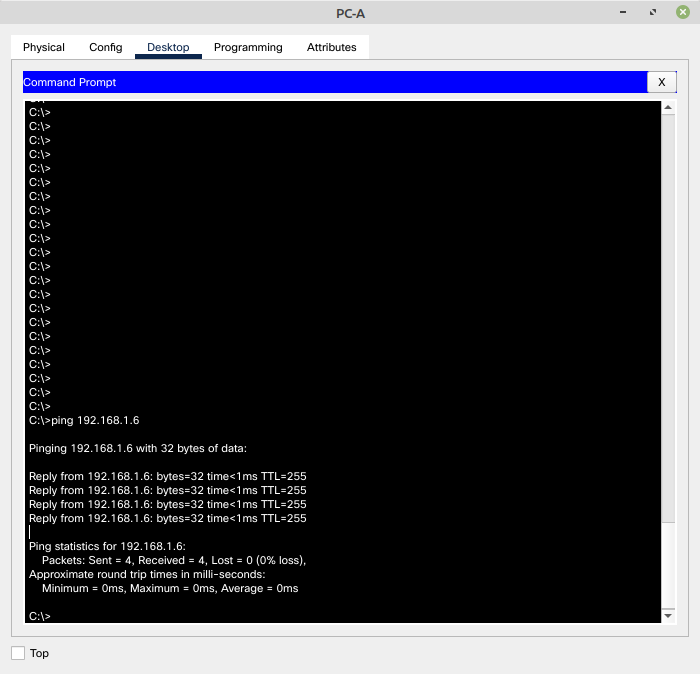
\includegraphics[width=0.6\linewidth]{images/pr8-ping-router}
		\caption{Эхо запрос на маршрутизатор \router}
		\label{fig:pr8-ping-router}
	\end{figure}
	
\end{step}

\end{mypart}

\begin{mypart}{Настройка маршрутизатора для доступа по протоколу SSH и
		обеспечение базовых мер безопасности}
	\begin{step}{Настройка аутентификации устройств}
		
		Перейдем в режим глобальной конфигурации.
		Зададим имя для маршрутизатора с помощью команды \texttt{hostname \router}.
		Зададим домен для устройства с помощью команды \texttt{ip domain-name cisco-lab.ru}
	\end{step}

	\begin{step}{Создание ключа шифрования с указанием его длины}
		
		Перейдем в режим глобальной конфигурации.
		Создадми ключ шифрования с помощью команды \texttt{crypto key generate rsa modulus 1024.}
	\end{step}

\begin{step}{Создание пользователя в локальной базе учетных записей}
	
	Перейдем в режим глобальной конфигурации.
	Создадим пользователя с помощью команды \texttt{username SSHadmin privilege 15 secret \\ Admin1p@55}.
\end{step}

\begin{step}{Активация протокола SSH на линиях VTY}
	
	Перейдем в режим конфигурации линии с помощью команды \texttt{line vty 0 4}.
	
	Активируем протокол SHH с помощью команды \texttt{transport input telnet ssh}.
	
	Изменим способ входа в систему таким образом, чтобы использовалась проверка пользователей
	по локальной базе учетных записей с помощью команды \texttt{login local}.
	
\end{step}

\begin{step}{Сохраните текущую конфигурацию в файл загрузочной конфигурации}
	
	Для сохранения конфигурации выполним комнаду \texttt{opy running-config startup-config}.
\end{step}

\begin{step}{Установка соединения с маршрутизатором по протоколу SSH}
	Установим соединение с маршрутизатором \router из командной строки компьютера PC-A (см. рисунок \ref{fig:pr8-ssh-to-router}).
	
	% TODO: \usepackage{graphicx} required
	\begin{figure}[h!]
		\centering
		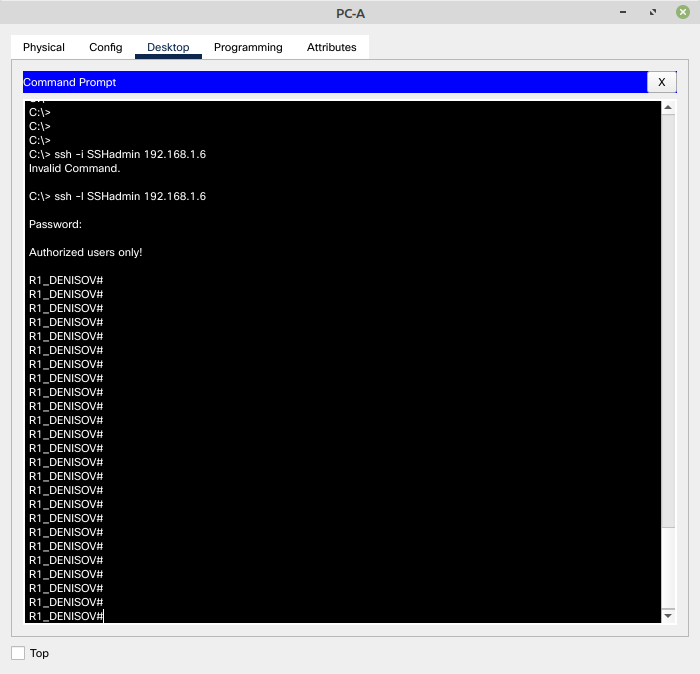
\includegraphics[width=0.6\linewidth]{images/pr8-ssh-to-router}
		\caption{Авторизация на маршрутизаторе \router по SHH}
		\label{fig:pr8-ssh-to-router}
	\end{figure}
	
	После совершения аутентификации видим приглашение для ввода привилегированного режима.
\end{step}


\begin{step}{Проверка соблюдения требований безопасности}


\q Подключитесь к маршрутизатору \router по протоколу Telnet. Разрешает ли \router
подключение по протоколу Telnet? Дайте пояснение.

\ans \textit{Подключение отклонено, потому что мы установили только SSH в качестве протокола соединения с маршрутизатором (см. рисунок \ref{fig:pr-8-telnet-abort})}. 

% TODO: \usepackage{graphicx} required
\begin{figure}
	\centering
	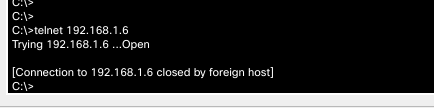
\includegraphics[width=0.6\linewidth]{images/pr-8-telnet-abort}
	\caption{Отклонение подключения к \router по протоколу telnet}
	\label{fig:pr-8-telnet-abort}
\end{figure}



\q Подключитесь к маршрутизатору \router по протоколу SSH. Разрешает ли \router
подключение по протоколу SSH?

\ans \textit{Да, подключение выполнено успешно (см. рисунок \ref{fig:pr8-ssh-to-router}).}


\q Намеренно укажите неверное имя пользователя и пароль, чтобы проверить, будет ли
заблокирован доступ к системе после двух неудачных попыток. Что произошло после ввода неправильных данных для входа в систему во второй раз?

\ans \textit{Возможность подключения заблокирована на 30 секунд после того, как в течение 120 секунд неправильные данные были введены больше 2 раз.}

\q Из сеанса подключения к маршрутизатору с помощью консоли отправьте команду \texttt{show login},
чтобы проверить состояние входа в систему. 


\ans % TODO: \usepackage{graphicx} required
\begin{figure}[h!]
	\centering
	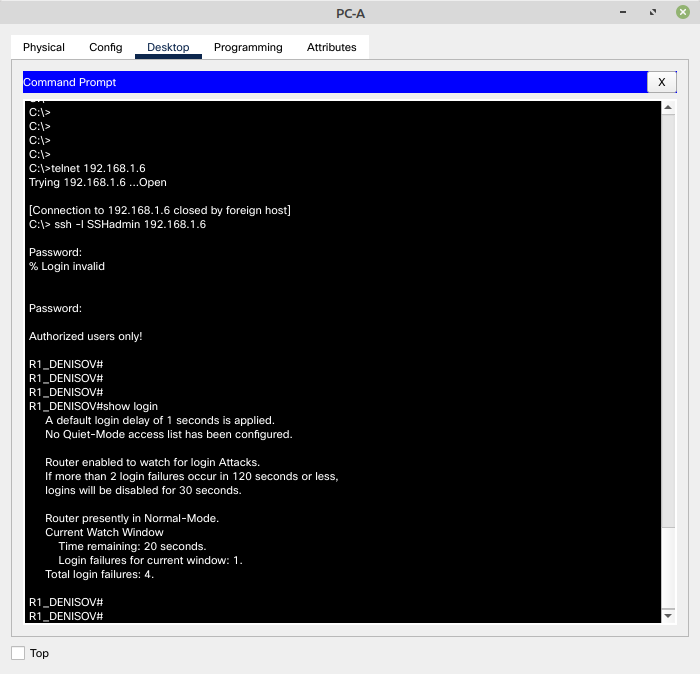
\includegraphics[width=0.6\linewidth]{images/pr8-show-login}
	\caption{Результат работы команды show login на маршрутизаторе \router}
	\label{fig:pr8-show-login}
\end{figure}

\q По истечении 30 секунд повторите попытку подключения к \router по протоколу SSH и
войдите в систему, используя имя SSHadmin и пароль Admin1p@55. Что отобразилось после успешного входа в систему?


\ans \textit{По истечении 30 секунд попытка авторизации на маршрутизаторе \router прошла успешно. Таймаут истек. 	После совершения аутентификации видим приглашение для ввода привилегированного режима.}

\q Войдите в привилегированный режим EXEC и введите в качестве пароля Enablep@55.
Если вы неправильно вводите пароль, прерывается ли сеанс SSH после двух неудачных попыток в
течение 120 секунд? Дайте пояснение.
\end{step}

\end{mypart}

\begin{mypart}{Настройка коммутатора для доступа по протоколу SSH и
		обеспечение базовых мер безопасности}
	
	\begin{step}{Настройте основные параметры коммутатора}
		
		По аналогии с маршрутизатором \router, настроим коммутатор \switch. Приведем его конфигурацию.
		
		\begin{lstlisting}
S1#show running-config 
Building configuration...

Current configuration : 1711 bytes
!
version 15.0
no service timestamps log datetime msec
no service timestamps debug datetime msec
service password-encryption
!
hostname S1
!
enable secret 5 $1$mERr$5wXi8fVAu3dNc0gNCjvIQ1
!
no ip domain-lookup
ip domain-name cisco-lab.ru
!
username SSHadmin secret 5 $1$mERr$uMzC7If3IbCZVifeGQ3rg/
!
spanning-tree mode pvst
spanning-tree extend system-id
!
interface FastEthernet0/1
!
interface FastEthernet0/2
shutdown
!
interface FastEthernet0/3
shutdown
!
interface FastEthernet0/4
shutdown
!
interface FastEthernet0/5
shutdown
!
interface FastEthernet0/6
shutdown
!
interface FastEthernet0/7
shutdown
!
interface FastEthernet0/8
shutdown
!
interface FastEthernet0/9
shutdown
!
interface FastEthernet0/10
shutdown
!
interface FastEthernet0/11
shutdown
!
interface FastEthernet0/12
shutdown
!
interface FastEthernet0/13
shutdown
!
interface FastEthernet0/14
shutdown
!
interface FastEthernet0/15
shutdown
!
interface FastEthernet0/16
shutdown
!
interface FastEthernet0/17
shutdown
!
interface FastEthernet0/18
shutdown
!
interface FastEthernet0/19
shutdown
!
interface FastEthernet0/20
shutdown
!
interface FastEthernet0/21
shutdown
!
interface FastEthernet0/22
shutdown
!
interface FastEthernet0/23
shutdown
!
interface FastEthernet0/24
shutdown
!
interface GigabitEthernet0/1
!
interface GigabitEthernet0/2
shutdown
!
interface Vlan1
ip address 192.168.1.16 255.255.255.0
!
banner motd ^CAuthorized users only!^C
!
!
!
line con 0
password 7 0822455D0A16
login
exec-timeout 5 0
!
line vty 0 4
exec-timeout 5 0
password 7 0822455D0A16
login local
transport input ssh
line vty 5 15
exec-timeout 5 0
password 7 0822455D0A16
login local
transport input ssh
!
end
		\end{lstlisting}
	\end{step}

	\begin{step}{Настройка коммутатора для соединения по протоколу SSH}
		
		
		По аналогии с маршрутизатором \router произведем настройку коммутатора \switch для соединения по протоколу SSH. 
		
		Перейдем в режим глобальной конфигурации.
		Зададим имя для маршрутизатора с помощью команды \texttt{hostname \router}.
		Зададим домен для устройства с помощью команды \texttt{ip domain-name cisco-lab.ru}.
		
		Создадми ключ шифрования с помощью команды \texttt{crypto key generate rsa modulus 1024 }.
	
		Создадим пользователя с помощью команды \texttt{username admin \\privilege 15 secret Enablep@55}.

		Перейдем в режим конфигурации линии с помощью команды \texttt{line vty 0 4}.
		
		Активируем протокол SHH с помощью команды \texttt{transport input telnet ssh}.

		Изменим способ входа в систему таким образом, чтобы использовалась проверка пользователей
		по локальной базе учетных записей с помощью команды \texttt{login local}.

	\end{step}

\begin{step}{Отключение неиспользуемых портов}
	
		Перейдем в режим глобальной конфигурации, затем в режим конфигурации множества интерфейсов с помощью команды \texttt{interface range FastEthernet0/2 - 24} и выключим их с помощью команды \texttt{shutdown}. После этого, все неиспользуемые порты будут отключены.
\end{step}

\begin{step}{Установка соединение с коммутатором по протоколу SSH}

	С компьютера PC-A установим подключение по протоколу SSH к интерфейсу SVI коммутатора S1.
	Подключение проведено успешно (см. рисунок \ref{fig:pr8-ssh-to-switch}), причем соединение по протоколу telnet отклоняется по соображениям безопасности.
	
	% TODO: \usepackage{graphicx} required
	\begin{figure}[h!]
		\centering
		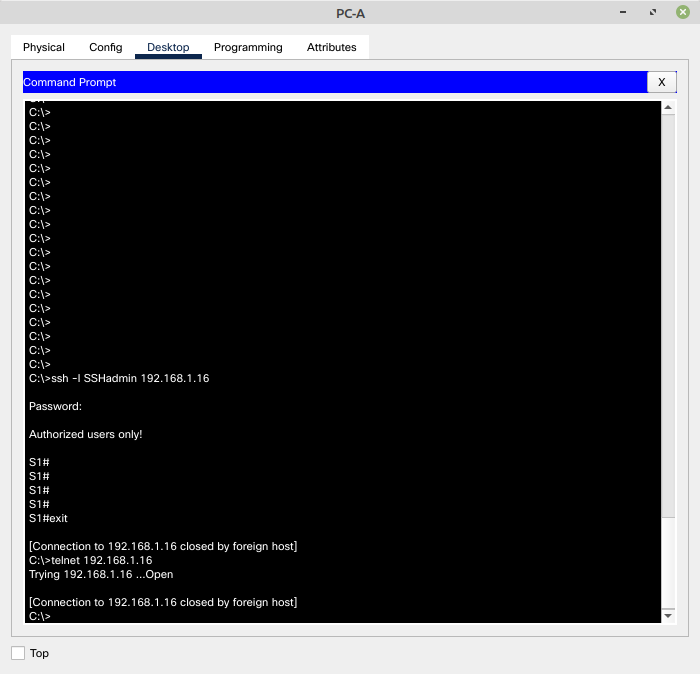
\includegraphics[width=0.6\linewidth]{images/pr8-ssh-to-switch}
		\caption{Соединение с коммутатором \switch по протоколу SSH}
		\label{fig:pr8-ssh-to-switch}
	\end{figure}
	
\end{step}

\begin{step}{Проверка мер безопасности}
	
	
Убедимся что протокол Telnet на коммутаторе отключен.

Подключимся к коммутатору по протоколу SSH и намеренно укажем неверное имя пользователя
и пароль, чтобы проверить, будет ли заблокирован доступ к системе.

По истечении 30 секунд повторим попытку подключения к \router по протоколу SSH и
войдем в систему, используя имя пользователя \textbf{SSHadmin} и пароль \textbf{Admin1p@55}.

\end{step}
\end{mypart}

\begin{mypart}{Настройка протокола SSH с использованием интерфейса
		командной строки (CLI) коммутатора}
	
	\begin{step}{Параметры для клиента SSH в Cisco IOS}
		
		Воспользуемся подсказкой <<?>> для команды \texttt{ssh} (см. рисунок \ref{fig:pr8-ssh-params}). 
		% TODO: \usepackage{graphicx} required
		\begin{figure}[h!]
			\centering
			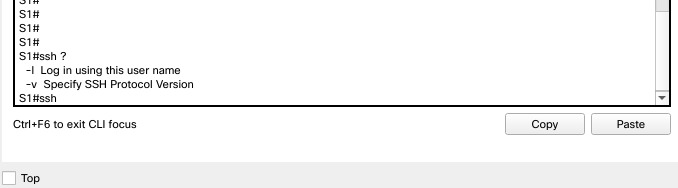
\includegraphics[width=0.5\linewidth]{images/pr8-ssh-params}
			\caption{Параметры команды ssh в Cisco IOS}
			\label{fig:pr8-ssh-params}
		\end{figure}
		
	\end{step}

\begin{step}{Установка соединения с маршрутизатором \router по
		протоколу SSH с коммутатора \switch}

Чтобы подключиться к маршрутизатору \router по протоколу SSH, введем команду \texttt{ssh –l SSHadmin 192.168.1.6.} Это позволит нам войти в систему под именем SSHadmin. При появлении
приглашения введите в качестве пароля \textbf{Admin1p@55} (см. рисунок \ref{fig:switch-ssh-router}).



% TODO: \usepackage{graphicx} required
\begin{figure}[h!]
	\centering
	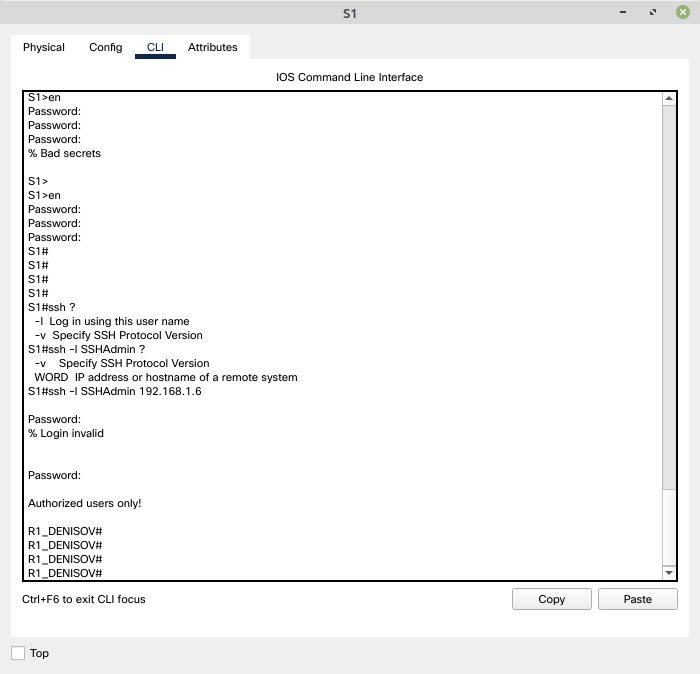
\includegraphics[width=0.6\linewidth]{images/switch-ssh-router}
	\caption{Установка соединения с маршрутизатором \router по
		протоколу SSH с коммутатора \switch}
	\label{fig:switch-ssh-router}
\end{figure}

\end{step}
\end{mypart}

\begin{mypart}{Защита лабораторной работы (ответ контрольные вопросы
		и вопросы преподавателя)}

\q Как предоставить доступ к сетевому устройству нескольким пользователям, у каждого из которых есть
собственное имя пользователя?

\ans \textit{Нужно настроить доступ по SSH и создать несколько пользователей на узле при
помощи команды \texttt{username}}.

\q Какие версии протокола SSH поддерживаются при использовании интерфейса командной строки?

\ans \textit{Существует две версии SSH, SSH версии 1 и SSH версии 2. Второй обеспечивает более высокий уровень безопасности.}
\end{mypart}



\end{document}



